\begin{frame}
	\frametitle{Das Klimasystem - Zusammenfassung}

	\begin{figure}
		\centering
		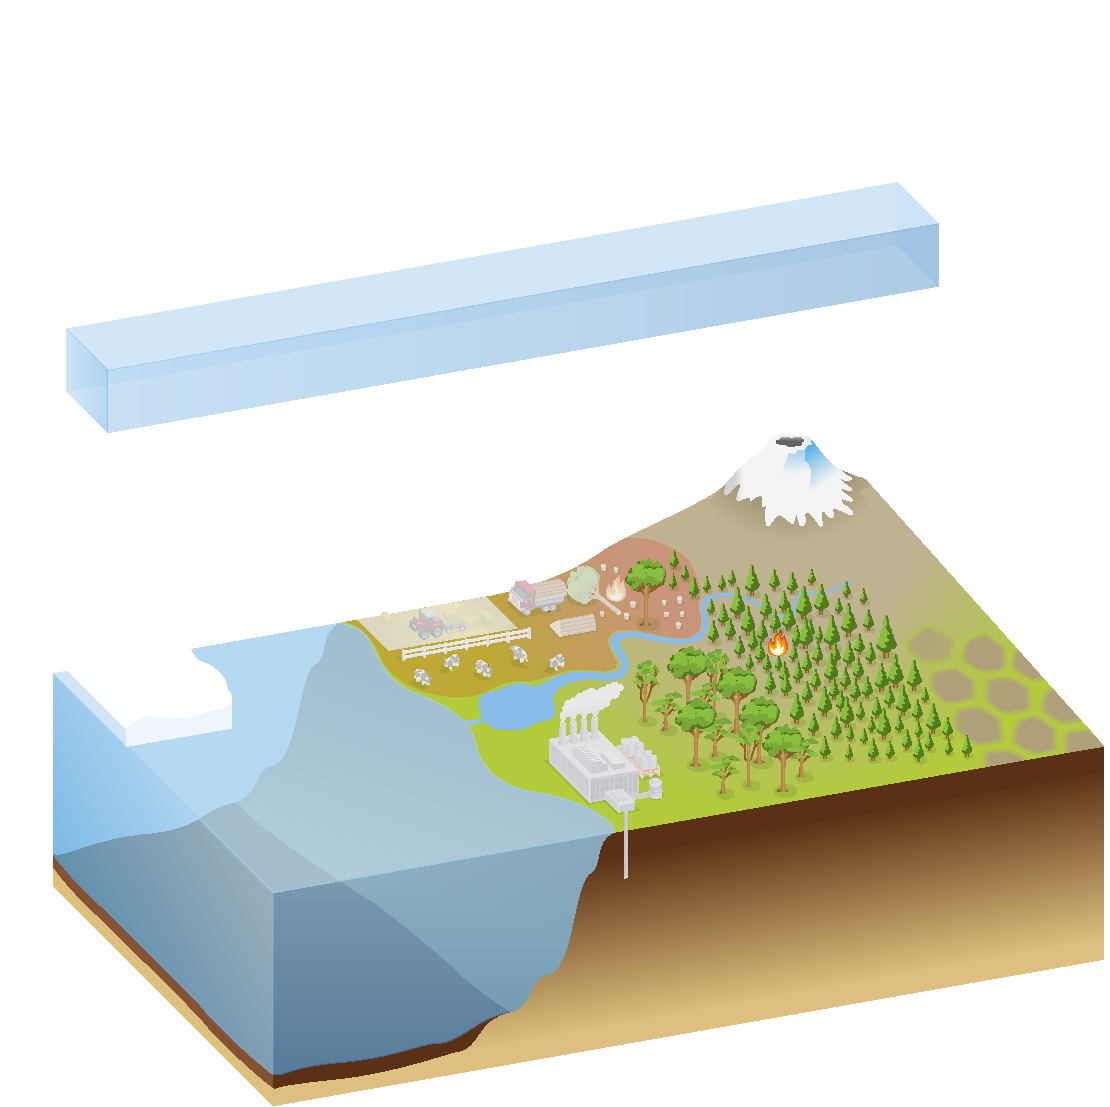
\includegraphics[trim={1cm 0cm 0cm 3cm}, clip, width=0.55\linewidth]{%
        bilder/climate_components/global_climate_components_spheres_ex_human.pdf}
		\caption{Abbildung des Klimasystems mit allen zuvor erklärten Elementen}
	\end{figure}

	\note{
		\begin{itemize}
			\item[] Abbildung mit allen zuvor erklärten Elementen
			\item[] das sind nur die größten Komponenten,
			\item[] viele kleinere Bereiche wie die Böden oder Elemente wie bestimmte Stoffkreisläufe sind ebenfalls wichtig
			\item[] es ist ein sehr komplexes System, an dem in vielen Stellen Änderungen und Wechselwirkungen auftreten
			\item[] also: komplexes System, mit komplexen Zusammenhängen
			\item[] in einzelnen Bereichen wie der Wolkenbildung sind noch Forschungsfragen offen
			\item[] (wir wollen Klarheit reinbringen, damit Lösungen eher im Kontext betrachtet werden können)
			\item[] (Eine Lösung kann nämlich Rückkopplungseffekte in anderen Bereichen erzeugen)
		\end{itemize}
	}
\end{frame}

\begin{frame}
	\frametitle{Das Klimasystem - Zusammenfassung}
	
	\begin{itemize}
		\item Das Klimasystem der Erde hat sehr viele verschiedene Komponenten
		\item Verständnis dieser erfordert Wissen in vielen Bereichen: Physik, Chemie, Biologie, Geologie und speziellere Disziplinen
		\item Vor allem können zwischen allen Teilen zahlreiche Wechselwirkungen auftreten
		\item Wird in Klimamodellen versucht ganzheitlich zu erfassen
		\item Modelle daher sehr komplex, können aber nie alles abbilden
		\begin{itemize}
			\item So viel wie nötig, so wenig wie möglich
			\item Bessere Modelle helfen menschlichen Einfluss auf das Klima genauer zu bestimmen
			\item Modelle verbessern sich mit der Zeit und Technik
			\item Grundlegende Aussagen ändern sich wenig
		\end{itemize}

	\end{itemize}
	
	\note{
		\begin{itemize}
			\item[] 
		\end{itemize}
	}
\end{frame}
